\documentclass[tikz,border=3mm]{standalone}
%\url{https://tex.stackexchange.com/q/532840/86}
\usetikzlibrary{knots,celtic}

\begin{document}
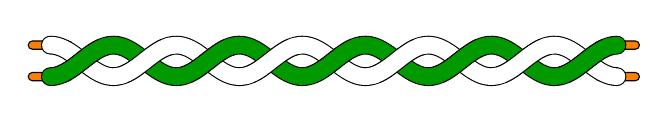
\begin{tikzpicture}[
  basic strand/.style={
    double=.,
    draw=black,
    looseness=1.2,
    double distance=6pt,
    line cap=round
  },
  crossing strand/.style={
    line width=6.8pt,
    only when rendering/.style={%
      draw=\pgfinnerstrokecolor,%
      line width=6pt,
      double=none,
    }
  }
]
\begin{knot}[%draft mode = crossings, % uncomment to see where the crossings are
  clip width = 1,
  flip crossing/.list={1,3,5,7,9},
  background color=black,
  only when rendering/.style={%
    basic strand
  },%
  every intersection/.style={
    crossing strand
  },
]
\path foreach \X in {0,4.5} {foreach \Y in {0.2,-0.2}
{(1.6*\X,\Y) node[draw,fill=orange,inner ysep=1.5pt,inner xsep=8pt,rounded
corners=1.5pt]{}}};
\strand[white]
     plot[domain=0:4.5,samples=251] (1.6*\x,{0.2*cos(\x*360)}); 
\strand[green!60!black]
   plot[domain=0:4.5,samples=251] (1.6*\x,{-0.2*cos(\x*360)}); 
\end{knot}
\end{tikzpicture}

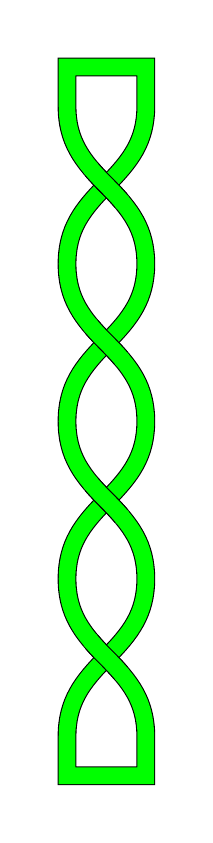
\begin{tikzpicture}[
  celtic path/.style={
    draw,
    double,
    black,
    double distance=6pt
  },
  celtic path 1/.style={
    double=white
  },
  celtic path 1/.style={
    double=green
  }
]
\CelticDrawPath{
  size={2,10}
}
\end{tikzpicture}
\end{document}
